\documentclass[a4paper]{article}
\usepackage[margin=3.5cm]{geometry}
\usepackage{amsmath}
\usepackage{amssymb}
\usepackage[svgnames]{xcolor}
\usepackage{amsthm}
\makeatletter
\def\th@plain{%
  \thm@notefont{}% same as heading font
  \itshape % body font
}
\def\th@definition{%
  \thm@notefont{}% same as heading font
  \normalfont % body font
}
\makeatother
\usepackage{dsfont}
\usepackage{graphicx}
\usepackage{caption}
\usepackage{hyperref}
\usepackage{cleveref}
\usepackage{datetime}
\usepackage{outlines}
\usepackage{float}
\usepackage{booktabs}
\usepackage{enumitem}
\usepackage{mathtools}
\usepackage{nicematrix}
\usepackage{nccmath}
\usepackage{lipsum}
\usepackage[activate={true,nocompatibility},final,tracking=true,kerning=true,spacing=true,factor=500,stretch=15,shrink=15]{microtype}

\addtolength{\skip\footins}{2mm}

\definecolor{fgcolor}{rgb}{0.345, 0.345, 0.345}
\newcommand{\hlnum}[1]{\textcolor[rgb]{0.686,0.059,0.569}{#1}}%
\newcommand{\hlstr}[1]{\textcolor[rgb]{0.192,0.494,0.8}{#1}}%
\newcommand{\hlcom}[1]{\textcolor[rgb]{0.678,0.584,0.686}{\textit{#1}}}%
\newcommand{\hlopt}[1]{\textcolor[rgb]{0,0,0}{#1}}%
\newcommand{\hlstd}[1]{\textcolor[rgb]{0.345,0.345,0.345}{#1}}%
\newcommand{\hlkwa}[1]{\textcolor[rgb]{0.161,0.373,0.58}{\textbf{#1}}}%
\newcommand{\hlkwb}[1]{\textcolor[rgb]{0.69,0.353,0.396}{#1}}%
\newcommand{\hlkwc}[1]{\textcolor[rgb]{0.333,0.667,0.333}{#1}}%
\newcommand{\hlkwd}[1]{\textcolor[rgb]{0.737,0.353,0.396}{\textbf{#1}}}%
\let\hlipl\hlkwb

\usepackage{framed}
\makeatletter
\newenvironment{kframe}{%
 \def\at@end@of@kframe{}%
 \ifinner\ifhmode%
  \def\at@end@of@kframe{\end{minipage}}%
  \begin{minipage}{\columnwidth}%
 \fi\fi%
 \def\FrameCommand##1{\hskip\@totalleftmargin \hskip-\fboxsep
 \colorbox{shadecolor}{##1}\hskip-\fboxsep
     % There is no \\@totalrightmargin, so:
     \hskip-\linewidth \hskip-\@totalleftmargin \hskip\columnwidth}%
 \MakeFramed {\advance\hsize-\width
   \@totalleftmargin\z@ \linewidth\hsize
   \@setminipage}}%
 {\par\unskip\endMakeFramed%
 \at@end@of@kframe}
\makeatother

\definecolor{shadecolor}{rgb}{.97, .97, .97}
\definecolor{messagecolor}{rgb}{0, 0, 0}
\definecolor{warningcolor}{rgb}{1, 0, 1}
\definecolor{errorcolor}{rgb}{1, 0, 0}
\newenvironment{knitrout}{}{} % an empty environment to be redefined in TeX


% code highlighting
\usepackage{minted}
\usepackage{xpatch}
\newminted[cminted]{python}{fontsize=\small}
\xpretocmd{\cminted}{\RecustomVerbatimEnvironment{Verbatim}{BVerbatim}{}}{}{}

% link coloring
\hypersetup{
   colorlinks,
   linkcolor={red!90!black},
   citecolor={green!40!black},
   urlcolor={blue!60!black}
}

% concatenation symbol (c.f. ++ in Haskell)
\newcommand\mdoubleplus{\mathbin{+\mkern-10mu+}}

% end of proof symbol
\newcommand{\newmarkedtheorem}[1]{%
  \newenvironment{#1}
    {\pushQED{\qed}\csname inner@#1\endcsname}
    {\popQED\csname endinner@#1\endcsname}%
  \newtheorem{inner@#1}%
}
% \renewenvironment{proof}{{\noindent\bfseries Proof.}}{*something*}
%\let\oldproofname=\proofname
%\renewcommand{\proofname}{\rm\bf{\oldproofname}}


\theoremstyle{definition}
%\newtheorem{eg}{Example}[section]
\newmarkedtheorem{eg}{Example}[section]
\newtheorem{remark}{Remark}
\theoremstyle{plain}
\newtheorem{define}{Definition\hspace{0.25em}\ignorespaces}
\newtheorem{property}{Property\hspace{0.25em}\ignorespaces}
\newtheorem{observation}{Observation}
\newtheorem{proposition}{Proposition}
\newtheorem{lemma}{Lemma\hspace{0.25em}\ignorespaces}
\newtheorem{corollary}{Corollary}
\newtheorem{theorem}{Theorem\hspace{0.25em}\ignorespaces}
\newtheorem{assump}{Assumption\hspace{0.25em}\ignorespaces}

\DeclareMathOperator{\interior}{int}

% cref settings
\crefname{equation}{equation}{equations}
\newcommand{\crefrangeconjunction}{--}

\newdateformat{monthyeardate}{\monthname[\THEMONTH] \THEYEAR}

\author{Jeroen van Riel} \date{\monthyeardate\today} \title{Vehicle trajectories
  in a tandem of intersections}

\begin{document}

\maketitle

\newcommand\halfopen[2]{\ensuremath{[#1,#2)}}
\newcommand\openhalf[2]{\ensuremath{(#1,#2]}}

\renewcommand{\labelitemii}{\textbullet}
\renewcommand{\labelitemiii}{\textbullet}


Let $\dot{x}(t)$ and $\ddot{x}(t)$ denote the first and second derivative of
$x(t)$ with respect to time $t$.
%
Let $\mathcal{D}[a,b]$ denote the set of valid \emph{trajectories}, which we
define as continuously differentiable functions $\gamma : [a,b] \rightarrow \mathbb{R}$
satisfying the constraints
\begin{align}
  0 \leq \dot{\gamma}(t) \leq 1 \quad \text{ and } \quad
  {-\omega} \leq \ddot{\gamma}(t) \leq \bar{\omega} , \quad \text{ for all } t \in [a,b] .
\end{align}
%
For $\gamma_{1} \in \mathcal{D}[a_{1}, b_{1}], \gamma_{2} \in \mathcal{D}[a_{2}, b_{2}]$, when
we write $\gamma_{1} \leq \gamma_{2}$ without explicitly mentioning where it applies, we mean
$t \in [a_{1}, b_{1}] \cap [a_{2}, b_{2}]$. We also write $\gamma \leq \min \{ \gamma_{1}, \gamma_{2} \}$ as a shorthand for
$\gamma \leq \gamma_{1}$ and $\gamma \leq \gamma_{2}$.

\begin{define}\label{def:stopping-trajectory}
  Given some trajectory $\gamma \in \mathcal{D}[a,b]$ and some time $\xi \in [a, b]$, consider the
  \emph{stopping trajectory} $\gamma[\xi]$ that is identical to the original trajectory until
  $\xi$, from where it starts decelerating to a full stop, so that at time
  $t \geq \xi$, the position is given by
\begin{subequations}
\begin{align}
  \gamma[\xi](t) &= \gamma(\xi) + \int_{\xi}^{t} \max\{0, \dot{\gamma}(\xi) - \omega(\tau-\xi) \} d\tau \\
                     &= \gamma(\xi) + \begin{cases}
                                        \dot{\gamma}(\xi)(t-\xi) - \omega(t-\xi)^{2} / 2 &\text{ for } t \leq \xi + \dot{\gamma}(\xi) / \omega , \\
                                        {(\dot{\gamma}(\xi))}^{2} / (2 \omega) &\text{ for } t \geq \xi + \dot{\gamma}(\xi) / \omega .
                                        \end{cases} \label{eq:underbound}
\end{align}
\end{subequations}
\end{define}

The above definition guarantees $\gamma[\xi] \in \mathcal{D}\halfopen{a}{\infty}$.
%
Note that a stopping trajectory serves as a lower bound in the sense that, for any
$\mu\in\mathcal{D}[c,d]$ such that $\gamma = \mu$ on $[a, \xi] \cap [c, d]$, we
have $\gamma \leq \mu$ and $\dot{\gamma} \leq \dot{\mu}$.
%
Furthermore, $\gamma[\xi](t)$ is a non-decreasing function in terms of either of its
arguments, while fixing the other. To see this for $\xi$, fix any $t$ and
consider $\xi_{1} \leq \xi_{2}$, then note that $\gamma[\xi_{1}](t)$ is a lower
bound for $\gamma[\xi_{2}](t)$.
%
\begin{property}
  Both $\gamma[\xi](t)$ and $\dot{\gamma}[\xi](t)$ are continuous when considered as functions
  of $(\xi, t)$.
\end{property}
\begin{proof}
  Write $f(\xi, t) := \gamma[\xi](t)$ to emphasize that we are dealing with two variables.
  Recall that $\dot{\gamma}$ is continuous by assumption, so the equation
  $\tau = \xi + \dot{\gamma}(\xi)/\omega$ defines a separation boundary of the
  domain of $f$. Both cases of~\eqref{eq:underbound} are continuous and they
  agree at this boundary, so $f$ is continuous on all of its domain.
  %
  Since $x \mapsto \max\{0, x \}$ is continuous, it is easy to see that also
  $(\xi, t) \mapsto \dot{\gamma}[\xi](t) = \max\{0, \dot{\gamma}(\xi) - \omega (\tau - \xi) \}$
  is continuous.
\end{proof}

Because $\gamma[\xi](t)$ is continuous and non-decreasing in $\xi$, the set
\begin{align}\label{eq:X}
  X(t_{0}, x_{0}) := \{\xi : \gamma[\xi](t_{0}) = x_{0}\}
\end{align}
is a closed interval (follows from Lemma~\ref{lemma:levelset}), so we can consider the maximum
\begin{align}\label{eq:xi}
  \xi(t_{0}, x_{0}) := \max X(t_{0}, x_{0}) .
\end{align}
%
Consider the closed region $\bar{U} := \{ (t, x) : \gamma[a](t) \leq x \leq \gamma[b](t) \}$.
For each $(t_{0}, x_{0}) \in \bar{U}$, there must be some $\xi_{0}$ such that
$\gamma[\xi_{0}](t_{0}) = x_{0}$, as a consequence of the intermediate value theorem and the
above continuity property.
%
Consider $\bar{U}$ without the points on $\gamma$, which we denote by
\begin{align}\label{eq:U}
  U := \bar{U} \setminus \{ (t,x) : \gamma(t) = x\}.
\end{align}
Next, we prove that $\gamma[\xi_{0}]$ is actually unique if $(t_{0}, x_{0}) \in U$, so that we
may regard $\xi(t_{0}, x_{0})$ as the canonical representation of this unique
trajectory $\gamma[\xi(t_{0}, x_{0})]$.

\begin{property}\label{prop:xi-unique}
  For $(t_{0}, x_{0}) \in U$, if
  $\gamma[\xi_{1}](t_{0}) = \gamma[\xi_{2}](t_{0}) = x_{0}$, then
  $\gamma[\xi_{1}] = \gamma[\xi_{2}]$.
\end{property}
\begin{proof}
  Suppose $t_{0} < \xi_{i}$, then $x_{0} = \gamma[\xi_{i}](t_{0}) = \gamma(t_{0})$ contradicts the assumption $(t_{0}, x_{0}) \in U$.
  %
  Therefore, assume $\xi_{1} \leq \xi_{2} < t_{0}$, without loss of generality.
  %
  Since $\gamma[\xi_{1}] = \gamma[\xi_{2}]$ on $[a, \xi_{1}]$, note that
  we have the lower bounds
  \begin{align}\label{eq:lowerbounds}
    \gamma[\xi_{1}] \leq \gamma[\xi_{2}] \quad \text{ and } \quad \dot{\gamma}[\xi_{1}] \leq \dot{\gamma}[\xi_{2}].
  \end{align}
  %
  We must have $\dot{\gamma}[\xi_{1}](t_{0}) = \dot{\gamma}[\xi_{2}](t_{0})$,
  because otherwise $\gamma[\xi_{1}] > \gamma[\xi_{2}]$ somewhere in a
  sufficiently small neighborhood of $t_{0}$, which contradicts the first lower
  bound.

  It is clear from Definition~\ref{def:stopping-trajectory} that
  \begin{align}
    \ddot{\gamma}[\xi_{i}](t) =
    \begin{cases}
      \ddot{\gamma}(t) & \text{ for } t < \xi_{i} , \\
      - \omega & \text{ for } t \in (\xi_{i}, \xi_{i} + \dot{\gamma}(\xi_{i})/\omega) , \\
      0 & \text{ for } t > \xi_{i} + \dot{\gamma}(\xi_{i})/ \omega ,
    \end{cases}
  \end{align}
  for both $i \in \{ 1, 2\}$.
  %
  Note that
  $\dot{\gamma}(\xi_{1}) - \omega(\xi_{2}-\xi_{1}) \leq \dot{\gamma}(\xi_{2})$,
  which can be rewritten as
  \begin{align}
    \xi_{2} + \dot{\gamma}(\xi_{2}) / \omega \geq \xi_{1} + \dot{\gamma}(\xi_{1}) / \omega .
  \end{align}
  This shows that $\ddot{\gamma}[\xi_{1}](t) \geq \ddot{\gamma}[\xi_{2}](t)$, for every
  $t \geq \xi_{2}$. Because
  $\dot{\gamma}[\xi_{1}](t_{0}) = \dot{\gamma}[\xi_{2}](t_{0})$, this in turn
  ensures that $\dot{\gamma}[\xi_{1}](t) \geq \dot{\gamma}[\xi_{2}](t)$ for $t \geq t_{0}$.
  Together with the opposite inequality in~\eqref{eq:lowerbounds}, we conclude
  that on $\halfopen{t_{0}}{\infty}$, we have $\dot{\gamma}[\xi_{1}] = \dot{\gamma}[\xi_{2}]$
  and thus $\gamma[\xi_{1}] = \gamma[\xi_{2}]$.

  It remains to show that $\gamma[\xi_{1}] = \gamma[\xi_{2}]$ on $[\xi_{1}, t_{0}]$, so consider the smallest
  $t^{*} \in (\xi_{1}, t_{0})$ such that $\gamma[\xi_{1}](t^{*}) < \gamma[\xi_{2}](t^{*})$.
  %
  Since $\dot{\gamma}[\xi_{1}] \leq \dot{\gamma}[\xi_{2}]$, this implies that $\gamma[\xi_{1}](t) < \gamma[\xi_{2}](t)$ for
  all $t \geq t^{*}$, but this contradicts the assumption $\gamma[\xi_{1}](t_{0}) = \gamma[\xi_{2}](t_{0})$.
\end{proof}

% previous argument of the above property
%
% Suppose we have $\xi_{1} \leq \xi_{2}$ such that $\gamma[\xi_{1}](\tau) = \gamma[\xi_{2}](\tau)$
% for some $\tau \geq \xi_{1}$, then we must have
% $\dot{\gamma}[\xi_{1}](\tau) = \dot{\gamma}[\xi_{2}](\tau)$, because otherwise
% $\gamma[\xi_{1}]$ and $\gamma[\xi_{2}]$ would be crossing at time $\tau$, which
% contradicts the fact that $\gamma[\xi_{1}]$ is a lower bound for $\gamma[\xi_{2}]$.
% Hence, $\gamma[\xi_{1}] = \gamma[\xi_{2}]$ for the whole domain
% $\halfopen{a}{\infty}$.
% %
% Such a situation occurs whenever $\xi_{1}$ and $\xi_{2}$ both lie in an
% interval where $\ddot{\gamma}(t) = -\omega$.


\begin{lemma}\label{lemma:curvejoining}
  Let $\gamma_{1} \in \mathcal{D}[a_{1}, b_{1}]$ and
  $\gamma_{2} \in \mathcal{D}[a_{2}, b_{2}]$ be two trajectories that are intersecting
  at exactly one time $t_{c}$ and assume
  $\dot{\gamma}_{1}(t_{c}) > \dot{\gamma}_{2}(t_{c})$,
  %Define $t_{f} := t_{c} + \dot{\gamma}_{1}(t_{c}) / \omega$,
  %denote the end of the deceleration of $\gamma_{1}[t_{c}]$,
  then under the conditions
  \begin{enumerate}[leftmargin=5em]
    \item[\normalfont(C1)\quad] $\gamma_{2} \geq \gamma_{1}[a_{1}]$,
    \item[\normalfont(C2)\quad] $b_{2} \geq t_{c} + \dot{\gamma}_{1}(t_{c}) / \omega$,
  \end{enumerate}
  there is a unique trajectory $\varphi$ such that
  \begin{enumerate}[label=(\roman*)\quad,leftmargin=5em]
    \item $\varphi = \gamma_{1}[\xi]$, for some $\xi < t_{c}$,
    \item $\varphi(\tau) = \gamma_{2}(\tau)$ and
          $\dot{\varphi}(\tau) = \dot{\gamma_{2}}(\tau)$, for some $\tau > t_{c}$,
    \item $\varphi \leq \gamma_{2}$.
  \end{enumerate}
\end{lemma}

\begin{figure}
  \centering
  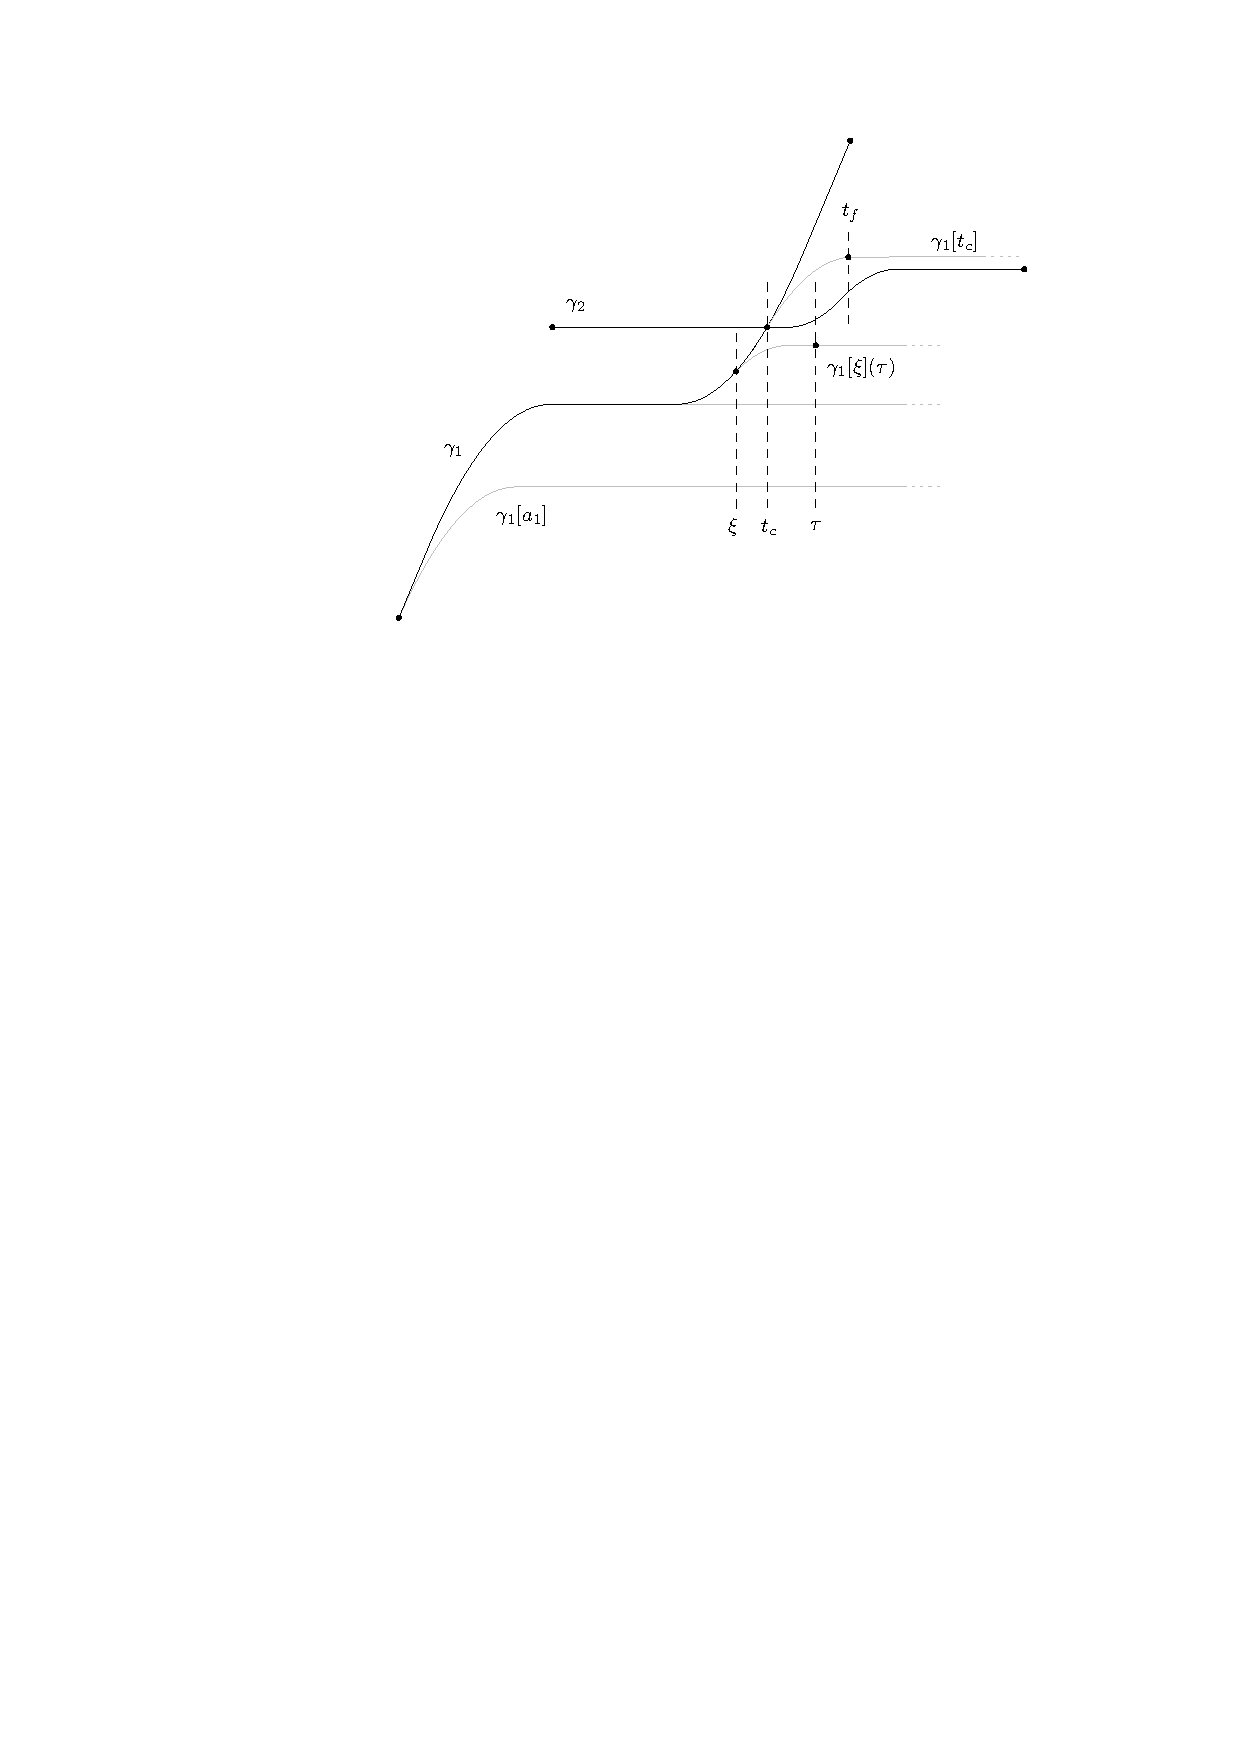
\includegraphics[scale=1.0]{figures/motion/rough/curvejoiningproof}
  \caption{Sketch of some quantities used in the proof of
    Lemma~\ref{lemma:curvejoining}, including some stopping trajectory
    candidates drawn in grey. The one satisfying the conditions of
    Lemma~\ref{lemma:curvejoining} is marked as $\varphi_{1}$. The little open
    dot halfway on $\gamma_{2}$ is refered to in Remark~\ref{rem:conditions}.}%
  \label{fig:proof}
\end{figure}

\begin{proof}

\phantom{.}
\begin{outline}

  % \1 Define $g$ such that $g(x, \tau) = \dot{\gamma}_{1}[\xi](\tau)$
  % for any $\xi$ such that $\gamma_{1}[\xi](\tau) = x$.

  % \2 Writing $h_{\tau}(\xi) := f_{x}(\xi, \tau)$, we define
  % $h_{\tau}^{-1}(x) := \{ \xi : f_{x}(\xi, \tau) = x \}$. Because this is the level set of a
  % continuous non-decreasing function, it must be a closed interval (Lemma~\ref{lemma:levelset}).
  % Hence, $g(x, \tau) := f_{v}(\max h_{\tau}^{-1}(x), \tau)$ is well-defined.

  \1 Identify for which parameters $\xi < t_{c} < \tau$ we have
  $\gamma_{1}[\xi](\tau) = \gamma_{2}(\tau)$ and $\dot{\gamma_{1}}[\xi](\tau) = \dot{\gamma}_{2}(\tau)$.

  \2 Define the set $U$ and the functions $X(t, x)$ and $\xi(t, x)$ as we did in
  \cref{eq:X,eq:xi,eq:U} for $\gamma$ above, but now for $\gamma_{1}$.

  \2 For each $\tau > t_{c}$, observe that $(\tau, \gamma_{2}(\tau)) \in U$. It follows
  from Property~\ref{prop:xi-unique} that
  $\varphi_{[\tau]} := \gamma_{1}[\xi(\tau, \gamma_{2}(\tau))]$ is the unique stopping trajectory such
  that $\varphi_{[\tau]}(\tau) = \gamma_{2}(\tau)$.
  %
  Next, we investigate when this unique trajectory touches $\gamma_{2}$
  tangentially. More precisely, consider the set of times
  \begin{align}
    T := \{ \tau > t_{c} : \dot{\varphi}_{[\tau]}(\tau) = \dot{\gamma}_{2}(\tau), \; \xi(\tau, \gamma_{2}(\tau)) < t_{c} \}.
  \end{align}

  \2 We define the auxiliary function $g(t, x) := \dot{\gamma}_{1}[\xi(t, x)](t)$,
  which gives the slope of the unique stopping trajectory through each point
  $(t, x) \in U$.

  \1 Function $g$ is continuous in $(t, x)$. We use the notation
  $N_{\varepsilon}(x) := (x - \varepsilon, x + \varepsilon)$.

  \2 We will write $f_{x}(\xi, t) = \gamma_{1}[\xi](t)$,
  $f_{v}(\xi, t) = \dot{\gamma}_{1}[\xi](t)$ and
  $h_{t}(\xi) = \gamma_{1}[\xi](t)$ to emphasize the quantities that we treat as
  variables. Observe that $h_{t}^{-1}(x) = X(t, x)$.

  \2 Let $x_{0} = f_{x}(\xi_{0}, \tau_{0})$ and $v_{0} = f_{v}(\xi_{0}, \tau_{0})$ for
  some $\xi_{0}$ and $\tau_{0}$ and pick some arbitrary $\varepsilon > 0$. Note that
  $\xi_{0} \in [\xi_{1}, \xi_{2}] := h_{\tau_{0}}^{-1}(x_{0})$.
  %
  We apply the $\varepsilon$-$\delta$ definition of continuity to each of these endpoints. Let
  $i \in \{1, 2\}$, then there exist $\delta_{i} > 0$ such that
  \begin{align}
  \xi \in N_{\delta_{i}}(\xi_{i}),\, \tau \in N_{\delta_{i}}(\tau_{0}) \implies
  f_{v}(\xi, \tau) \in N_{\varepsilon}(v_{0}).
  \end{align}
  Let $\delta = \min\{ \delta_{1}, \delta_{2} \}$ and define $N_{1} := (\xi_{1} - \delta, \xi_{2} + \delta)$
  and $N_{2} := N_{\delta}(\tau_{0})$, then
  \begin{align}
  \xi \in N_{1},\, \tau \in N_{2} \implies f_{v}(\xi, \tau) \in N_{\varepsilon}(v_{0}) .
  \end{align}

  This is obvious when $\xi$
  is chosen to be in one of $N_{\delta_{i}}(\xi_{i})$. Otherwise, we must have $\xi \in [\xi_{1}, \xi_{2}]$,
  in which case $f_{v}(\xi, \tau) = f_{v}(\xi_{1}, \tau) \in N_{\varepsilon}(v_{0})$.

  \2 Because $h_{\tau_{0}}(\xi)$ is continuous, the image $I := h_{\tau_{0}}(N_{1})$
  must be an interval containing $x_{0}$, with
  $\inf I = h_{\tau_{0}}(\xi_{1} - \delta)$ and
  $\sup I = h_{\tau_{0}}(\xi_{2} + \delta)$.
  %
  We argue that $I$ contains $x_{0}$ in its interior. For sake of
  contradiction, suppose $x_{0} = \max I$, then $h_{\tau_{0}}(\xi_{2} + \delta') = x_{0}$,
  for each $\delta' \in (0, \delta)$, because $h_{\tau_{0}}$ is non-decreasing, but this
  contradicts the definition of $\xi_{2}$. Similarly, when $x_{0} = \min I$, then
  $h_{\tau_{0}}(\xi_{1} - \delta') = x_{0}$, for each $\delta' \in (0, \delta)$, which contradicts the
  definition of $\xi_{1}$.

  \2 Define $\nu := \min \{ x_{0} - \inf I, \sup I - x_{0}\}$ and
  $N_{3} := (x_{0} - \nu / 2, x_{0} + \nu / 2)$. Because $h_{\tau}(\xi)$ is also
  continuous in $\tau$, there exists a neighborhood $N_{2}^{*} \subset N_{2}$ of
  $\tau_{0}$ such that for every $\tau \in N_{2}^{*}$, we have
  \begin{align*}
  &h_{\tau}(\xi_{1} - \delta) \leq h_{\tau_{0}}(\xi_{1} - \delta) + \nu/2 = \inf I + \nu /2 < x_{0} - \nu/2 , \\
  &h_{\tau}(\xi_{2} + \delta) \geq h_{\tau_{0}}(\xi_{2} + \delta) - \nu/2 = \sup I - \nu /2 > x_{0} + \nu/2 ,
  \end{align*}
  which shows that $h_{\tau}(N_{1}) \supset N_{3}$. It follows that
  $h_{\tau}^{-1}(N_{3}) \subset N_{1}$.

  \2 Finally, take any $\tau \in N_{2}^{*}$ and $x \in N_{3}$, then there exists
  some $\xi \in N_{1}$ such that $h_{\tau}(\xi) = x$ and
  $g(\tau, x) = f_{v}(\max h_{\tau}^{-1}(x), \tau) = f_{v}(\xi, \tau) \in N_{\varepsilon}(v_{0})$.

  \1 Function $g$ is non-decreasing and Lipschitz continuous in $x$.

  \2 Let $x_{1} \leq x_{2}$ and $\tau$ such that $g(\tau, x_{1})$ and
  $g(\tau, x_{2})$ are defined. There must be $\xi_{1} \leq \xi_{2}$ such that
  $h_{\tau}(\xi_{1}) = x_{1}$ and $h_{\tau}(\xi_{2}) = x_{2}$ and we have
  \begin{align*}
    g(\tau, x_{1}) = \dot{\gamma}_{1}[\xi_{1}](\tau)
    &= \max\{0, \dot{\gamma}_{1}(\xi_{1}) - \omega(\tau - \xi_{1}) \} \\
    &= \max\{0, \dot{\gamma}_{1}(\xi_{1}) - \omega(\xi_{2} - \xi_{1}) - \omega(\tau - \xi_{2}) \} \\
    &\leq \max\{0, \dot{\gamma}_{1}(\xi_{2}) - \omega(\tau - \xi_{2}) \}
    = \dot{\gamma}_{1}[\xi_{2}](\tau) = g(\tau, x_{2}) .
  \end{align*}

  \2 Furthermore, we have
  $\dot{\gamma}_{1}(\xi_{2}) \leq \dot{\gamma}_{1}(\xi_{1}) + \bar{\omega}(\xi_{2} - \xi_{1})$,
  so that
  \begin{align*}
    g(\tau, x_{2}) &= \max\{0, \dot{\gamma}_{1}(\xi_{2}) - \omega(\tau - \xi_{2}) \} \\
              &\leq \max\{0, \dot{\gamma}_{1}(\xi_{1}) + \bar{\omega}(\xi_{2} - \xi_{1}) - \omega(\tau - \xi_{2}) \} \\
              &= \max\{0, \dot{\gamma}_{1}(\xi_{1}) - \omega(\tau-\xi_{1}) + (\omega + \bar{\omega})(\xi_{2} - \xi_{1}) \} \\
              &\leq \max\{0, \dot{\gamma}_{1}(\xi_{1}) - \omega(\tau - \xi_{1}) \} + (\omega + \bar{\omega})(\xi_{2} - \xi_{1}) \\
              &= g(\tau, x_{1}) + (\omega + \bar{\omega})(\xi_{2} - \xi_{1}) .
  \end{align*}
  Observe that, together with the above non-decreasing property, this shows that
  $g$ is Lipschitz continuous in $x$, with Lipschitz constant
  $(\omega + \bar{\omega})$.

  \1 Note that $T$ can also be written as
  \begin{align}
    T = \{ \tau > t_{c} : g(\tau, \gamma_{2}(\tau)) = \dot{\gamma}_{2}(\tau), \; \xi(\tau, \gamma_{2}(\tau)) < t_{c} \} ,
  \end{align}
  so continuity of $g$ shows that it is a closed set (Lemma~\ref{lemma:levelset}). It is not
  necessarily connected (see for example Figure~\ref{fig:proof}), so it is the
  union of a sequence of disjoint closed intervals $T_{1}, T_{2}, \dots, T_{n}$.

  \2 Define $\tau_{i} := \min \, T_{i}$ and let $\varphi_{i} := \varphi_{[\tau_{i}]}$
  denote the unique stopping trajectory through $(\tau_{i}, \gamma_{2}(\tau_{i}))$.
  %
  For $\tau \in T_{i}$, we have
  $\dot{\gamma}_{2}(\tau) = g(\tau, \gamma_{2}(\tau))$ by definition of $T_{i}$.
  %
  Moreover, we have
  \begin{align}\label{eq:phi-tangent}
    \dot{\varphi}_{i}(t) = g(t, \varphi_{i}(t)),
  \end{align}
  for every $t$ for which these quantities are defined, so in particular on $T_{i}$.
  %
  This shows that $\gamma_{2}$ and $\varphi_{i}$ are both solutions to the initial value problem
  \begin{align}
    \begin{cases}
      \,\dot{x}(t)\, = g(t, x(t)) \;  \text{ for } t \in T_{i} , \\
      x(\tau_{i}) = \gamma_{2}(\tau_{i}) .
    \end{cases}
  \end{align}
  %
  Since $g(t, x)$ is continuous in $t$ and Lipschitz continuous in $x$, it is a
  consequence of the (local) existence and uniqueness theorem
  (Picard-Lindel{\"o}f) that $\gamma_{2} = \varphi_{i}$ on $T_{i}$.
  %
  Hence, we have $\varphi_{i} = \varphi_{[\tau]}$ for any $\tau \in T_{i}$, so we regard
  $\varphi_{i}$ as being the canonical stopping trajectory for $T_{i}$.

  % Let $\tau'$ be the largest $\tau \in T_{i}$ such that
  % $\gamma_{2}(\tau) = \varphi_{i}(\tau)$. Suppose $\tau' < \hat{\tau}_{i}$, then by
  % the existence and uniqueness theorem (Picard-Lindel{\"o}f) there exists a
  % unique solution of the initial value problem
  % \begin{align*}
  %   \dot{\phi}(t) = g(t, \phi(t)), \quad \phi(\tau') = \gamma_{2}(\tau')
  % \end{align*}
  % on the interval $[\tau' - \delta, \tau' + \delta]$ for some $\delta > 0$.
  %
  % But $\varphi_{i}$ is a solution, so
  % $\varphi_{i}(\tau' + \delta) = \gamma_{2}(\tau' + \delta)$ for some sufficiently
  % small $\delta > 0$, but this contradicts the definition of $\tau'$. Therefore,
  % $\tau' = \hat{\tau}_{i}$.

  \1 Show that $\tau_{1}$ and thus $\varphi_{1}$ exists. We write
  $s(\tau) := g(\tau, \gamma_{2}(\tau))$ and
  $t_{f} := t_{c} + \dot{\gamma}_{1}(t_{c}) / \omega$. Note that this part
  relies on conditions (C1) and (C2).

  \2 Suppose $\gamma_{2}(t_{f}) \leq \gamma_{1}[t_{c}](t_{f})$, then it follows from the fact
  that $g$ is non-decreasing in $x$ that
  $g(t_{f}, \gamma_{2}(t_{f})) \leq g(t_{f}, \gamma_{1}[t_{c}](t_{f})) = \dot{\gamma}_{1}(t_{c}) - \omega(t_{f} - t_{c}) = 0$,
  so $s(t_{f}) = 0$.

  \2 Otherwise $\gamma_{2}(t_{f}) > \gamma_{1}[t_{c}](t_{f})$, then it follows
  (from Lemma \dots) that $\gamma_{2}$ crosses $\gamma_{1}[t_{c}]$ at some time
  $t_{d} \in (t_{c}, t_{f})$ with
  $\dot{\gamma}_{2}(t_{d}) > \gamma_{1}[t_{c}](t_{d}) = s(t_{d})$.

  \2 We have $\gamma_{1}[a_{1}](t) \leq \gamma_{2}(t) \leq \gamma_{1}[t_{c}](t)$ for
  $t \in \{ t_{f}, t_{d} \}$, so the intermediate value theorem guarantees that
  $s(t)$ actually exists in both cases, because there is some
  $a_{1} \leq \xi < t_{c}$ such that $\gamma_{2}(t) = \gamma_{1}[\xi](t)$ and thus
  $s(t) = g(t, \gamma_{2}(t)) = \dot{\gamma}_{1}[\xi](t)$ exists.

  \2 In both cases above, we have
  $\dot{\gamma}_{2}(t_{c}) < \dot{\gamma}_{1}(t_{c}) = s(t_{c})$ and
  $\dot{\gamma}_{2}(t_{d}) \geq s(t_{d})$ for some $t_{d} \in \openhalf{t_{c}}{t_{f}}$.
  Hence, there must be some smallest $\tau_{1} \in \openhalf{t_{c}}{t_{d}}$ such that
  $\dot{\gamma_{2}}(\tau_{1}) = s(\tau_{1})$, which is a consequence of the intermediate
  value theorem.

  \1 If $i \geq 2$, then $\varphi_{i} > \gamma_{2}$ somewhere.

  \2 Let $i \geq 1$, we show that $\varphi_{i+1}(t) > \gamma_{2}(t)$ for some $t$.
  %
  Recall the lower bound property, so $\gamma_{2}(t) \geq \varphi_{i}(t)$ and
  $\dot{\gamma}_{2}(t) \geq \dot{\varphi}_{i}(t)$ for $t \geq \tau_{i}$.
  %
  Define $\hat{\tau}_{i} := \max \, T_{i}$, such that
  $T_{i} = [\tau_{i}, \hat{\tau}_{i}]$, then by definition of $T_{i}$, there
  must be some $\delta > 0$ such that
  \begin{align}
    \gamma_{2}(\hat{\tau}_{i} + \delta) > \varphi_{i}(\hat{\tau}_{i} + \delta) ,
  \end{align}
  since otherwise $\gamma_{2} = \varphi_{i}$ on some open neighborhood of
  $\hat{\tau}_{i}$ and then also
  \begin{align}
    \dot{\gamma}_{2}(t) = \dot{\varphi}_{i}(t) \overset{\text{\eqref{eq:phi-tangent}}}{=} g(t, \varphi_{i}(t)) = g(t, \gamma_{2}(t)),
  \end{align}
  which contradicts the definition of $\hat{\tau}_{i}$.
  %
  Therefore, we have $\gamma_{2}(t) > \varphi_{i}(t)$ for all $t \geq \hat{\tau}_{i} + \delta$. For
  $t = \tau_{i+1}$, in particular, it follows that
  $\varphi_{i+1}(\tau_{i+1}) = \gamma_{2}(\tau_{i+1}) > \varphi_{i}(\tau_{i+1})$, which shows that
  $\varphi_{i+1} > \varphi_{i}$ on $(\xi_{i}, \infty)$, due to Property~\ref{prop:xi-unique}, but this means that
  $\varphi_{i+1}(\tau_{i}) > \varphi_{i}(\tau_{i}) = \gamma_{2}(\tau_{i})$.

  \1 If $\varphi_{i} > \gamma_{2}$ somewhere, then $i \geq 2$.

  \2 Suppose $\varphi_{i}(t_{x}) > \gamma_{2}(t_{x})$ for some
  $t_{x} \in (t_{c}, \tau_{i})$, then there must be some
  $\tau_{0} \in (t_{c}, t_{x})$ such that
  $\gamma_{2}(\tau_{0}) = \varphi_{i}(\tau_{0})$ and
  $\dot{\gamma}_{2}(\tau_{0}) < \dot{\varphi}(\tau_{0})$. Note that this
  crossing must happen because we require $\xi_{i} < t_{c}$.

  \2 Since $g(t, x)$ is non-decreasing in $x$, we have
  \begin{align}
    s(t) = g(t, \gamma_{2}(t)) \leq g(t, \varphi_{i}(t)) = \dot{\varphi}_{i}(t) ,
  \end{align}
  for every $t \in [\tau_{0}, \tau_{i}]$ and at the endpoints, we have
  \begin{align}
    s(\tau_{0}) = \varphi_{i}(\tau_{0}), \quad s(\tau_{i}) = \varphi_{i}(\tau_{i}) .
  \end{align}
  %
  Furthermore, observe that $\gamma_{2}(\tau_{0}) = \varphi_{i}(\tau_{0})$ and
  $\gamma_{2}(\tau_{i}) = \varphi_{i}(\tau_{i})$ require that
  \begin{align}\label{eq:distance-traveled}
    \int_{\tau_{0}}^{\tau_{i}} \dot{\gamma}_{2}(t) dt  = \int_{\tau_{0}}^{\tau_{i}} \dot{\varphi}_{i}(t) dt .
  \end{align}

  \2 Since $\dot{\gamma}_{2}(\tau_{0}) < \dot{\varphi}_{i}(\tau_{0})$, it follows
  from~\eqref{eq:distance-traveled} that there must be some $t \in (\tau_{0}, \tau_{i})$
  such that $\dot{\gamma}_{2}(t) > \dot{\varphi}_{i}(t)$.
  %
  Together with $s(\tau_{0}) = \dot{\varphi}_{i}(\tau_{0}) > \dot{\gamma}_{2}(\tau_{0})$
  and $s(t) \leq \dot{\varphi}_{i}(t)$ for $t \in [\tau_{0}, \tau_{i}]$, this means there is some $\tau^{*}$ such
  that $\dot{\gamma}_{2}(\tau^{*}) = s(\tau^{*})$, again as a consequence of the
  intermediate value theorem. Therefore, $\tau^{*} \in T_{j}$ for some $j < i$, which
  shows that $i \geq 2$.


  \1 The above two points establish that $\varphi_{i} \leq \gamma_{2}$ if and only if $i=1$.
  To conclude, we have shown that $\varphi := \varphi_{1}$ exists and is the unique
  trajectory satisfying the stated requirements with $\tau = \tau_{i}$ and
  $\xi = \xi(\tau_{i}, \gamma_{2}(\tau_{i}))$. \qedhere
\end{outline}
\end{proof}


\begin{figure}
  \centering
  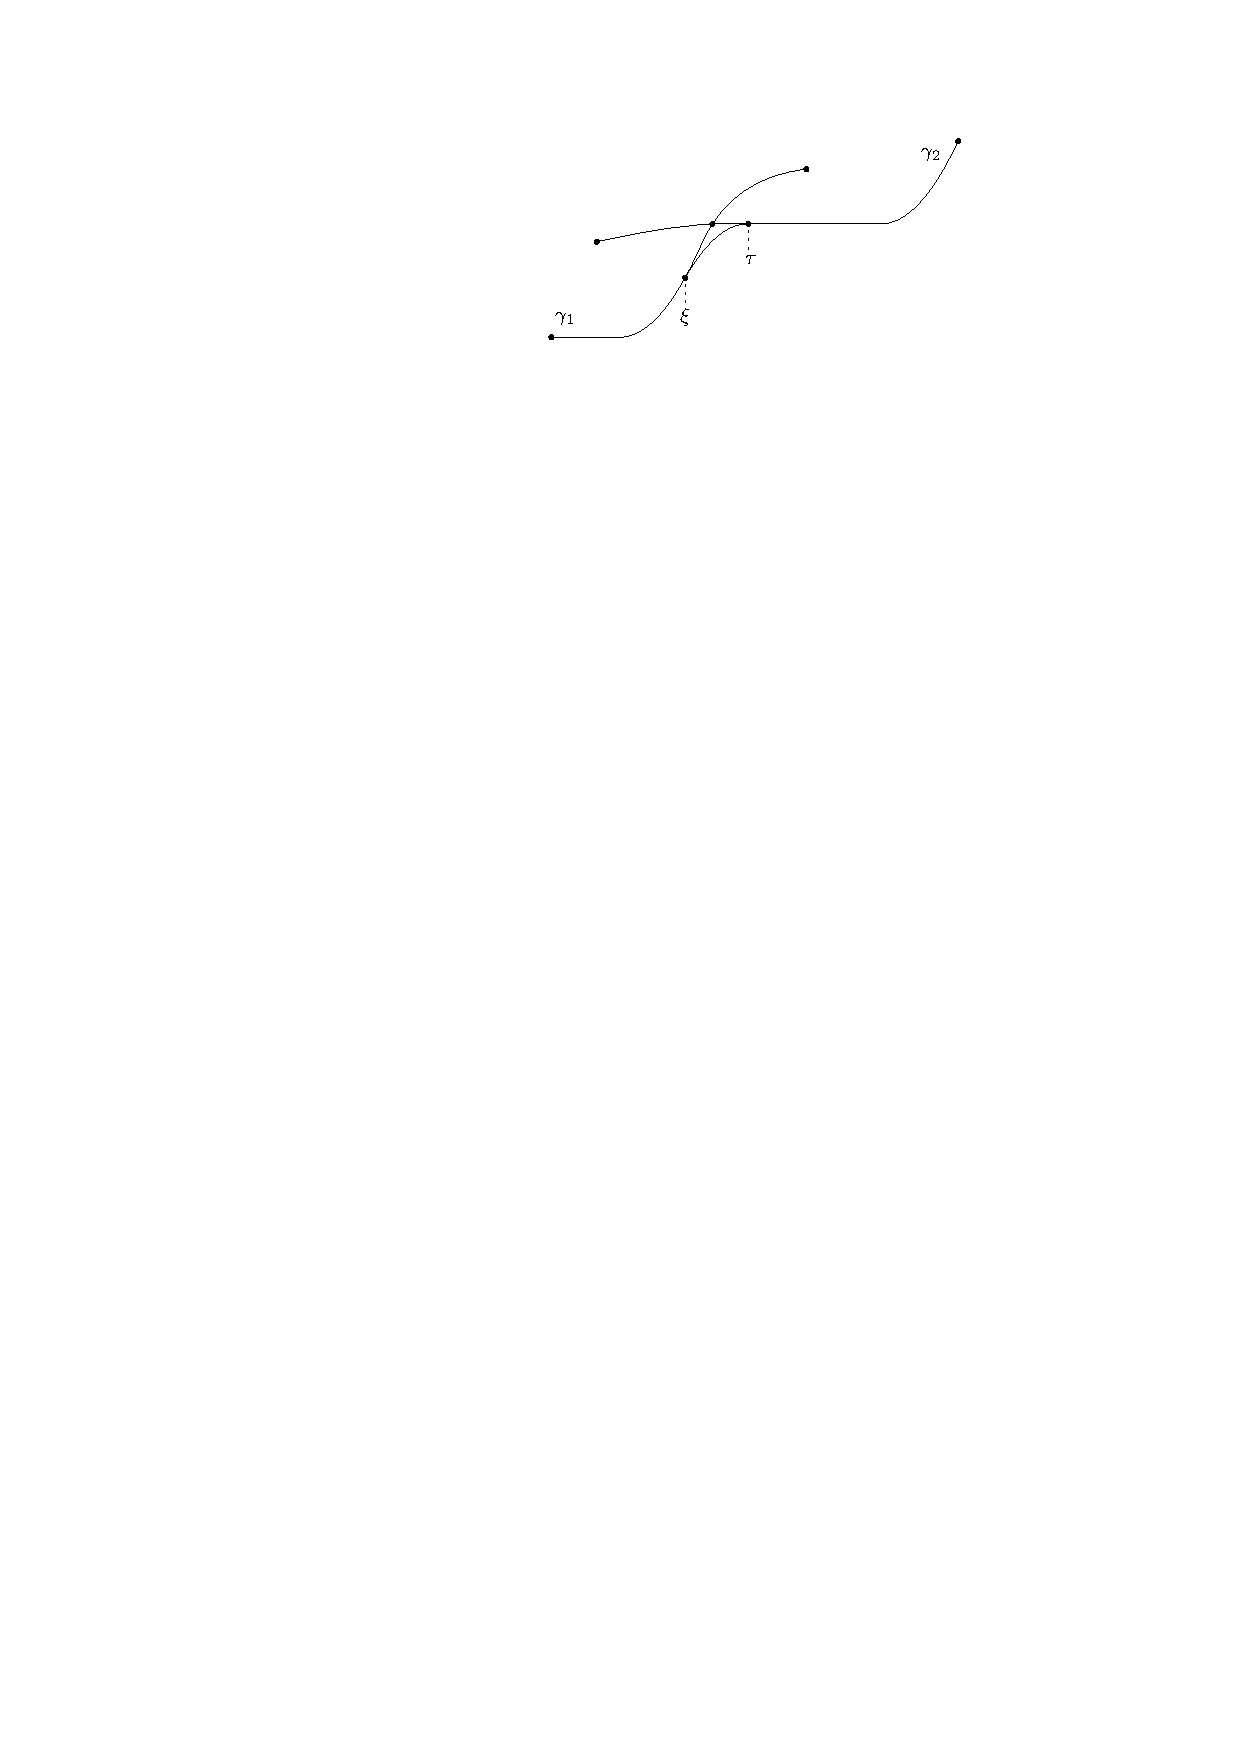
\includegraphics[scale=1]{figures/motion/rough/curvejoining}
  \caption{Two intersecting trajectories joined together by a part of a stopping
    trajectory.}%
  \label{fig:curvejoining}
\end{figure}

\begin{remark}\label{rem:conditions}
  It is easy to see that condition (C1) in Lemma~\ref{lemma:curvejoining} is necessary. Suppose there
  is some $t_{x} \in (t_{c}, \infty)$ such that
  $\gamma_{1}[a_{1}](t_{x}) > \gamma_{2}(t_{x})$, then for any other
  $\xi \in (a_{1}, t_{c})$, we have $\gamma_{1}[\xi](t_{x}) > \gamma_{2}(t_{x})$
  as well, due to the lower bound property of stopping trajectories, so
  requirement \textit{(iii)} is violated.
  %
  Condition (C2) is not necessary, which can be seen from stopping trajectory
  $\varphi_{1}$ in Figure~\ref{fig:proof}, which satisfies the conditions, but
  would also have been valid if $\gamma_{2}$ ended somewhat earlier than
  $t_{f}$, for example until the open dot.
\end{remark}

Suppose we have two trajectories that cross each other exactly once.
Lemma~\ref{lemma:curvejoining} gives conditions under which, roughly speaking,
these trajectories can be glued together to form a smooth trajectory by
introducing a stopping trajectory in between, as illustrated in Figure~\ref{fig:curvejoining}.
%
Suppose we have two trajectories $\gamma_{1} \in \mathcal{D}[a_{1}, b_{1}]$ and
$\gamma_{2} \in \mathcal{D}[a_{2}, b_{2}]$ that are intersecting at exactly a
single time $t_{c}$. We are looking for some trajectory $\psi$ that satisfies
$\psi \in \mathcal{D}[a_{1}, b_{2}]$ and
$\psi \leq \min\{\gamma_{1}, \gamma_{2}\}$.
%
When the two trajectories intersect tangentially, i.e., with equal derivatives
at $t_{c}$, it is clear that $\min\{\gamma_{1}, \gamma_{2}\}$ is the unique
trajectory satisfying these requirements. When the intersection is not
tangentially, it follows from Lemma~\ref{lemma:curvejoining} that $\psi$ is
given by
\begin{align}
  \psi(t) =
  \begin{cases}
    \gamma_{1}(t) & \text{ for } t < \tau , \\
    \varphi(t) & \text{ for } t \in [\tau, \xi] , \\
    \gamma_{2}(t) & \text{ for } t > \xi ,
  \end{cases}
\end{align}
where $\varphi$ and $(\tau,\xi)$ are as given by
Lemma~\ref{lemma:curvejoining}.
%
To conclude, the above discussion motivates and justifies the following
definition.

\begin{define}
  Let $\gamma_{1} \in \mathcal{D}[a_{1}, b_{1}]$ and
  $\gamma_{2} \in \mathcal{D}[a_{2}, b_{2}]$ and suppose they intersect at
  exactly a single time $t_{c}$. We write $\gamma_{1} * \gamma_{2}$ to denote
  the unique trajectory that satisfies
  $\gamma_{1} * \gamma_{2} \in \mathcal{D}[a_{1}, b_{2}]$ and
  $\gamma_{1} * \gamma_{2} \leq \min\{\gamma_{1}, \gamma_{2}\}$.
\end{define}

\begin{lemma}
  Let $\gamma_{1} \in \mathcal{D}[a_{1}, b_{2}]$ and
  $\gamma_{2} \in \mathcal{D}[a_{2}, b_{2}]$ be such that $\gamma_{1} * \gamma_{2}$ exists. All
  trajectories $\gamma \in \mathcal{D}[a, b]$ that are such that
  $\gamma \leq \min\{\gamma_{1}, \gamma_{2}\}$, must satisfy $\gamma \leq \gamma_{1} * \gamma_{2}$.
\end{lemma}
\begin{proof}
  Write $\psi := \gamma_{1} * \gamma_{2}$ as a shorthand. We obviously have
  $\gamma \leq \psi$ on $[a_{1}, \xi] \cup [\tau, b_{2}]$, so consider the interval $(\xi, \tau)$ of the joining
  deceleration part. Suppose there exists some $t_{d} \in (\xi, \tau)$ such that
  $\gamma(t_{d}) > \psi(t_{d})$. Because $\gamma(\xi) \leq \psi(\xi)$, this means that $\gamma$ must
  intersect $\psi$ at least once in $\halfopen{\xi}{t_{d}}$, so let
  $t_{c} := \sup \, \{ t \in \halfopen{\xi}{t_{d}} : \gamma(t) = \psi(t) \}$ be the latest
  time of intersection such that $\gamma \geq \psi$ on $[t_{c}, t_{d}]$. There must be
  some $t_{c} \in [t_{c}, t_{d}]$ such that $\dot{\gamma}(t_{v}) > \dot{\psi}(t_{v})$, otherwise
  \begin{align*}
    \gamma(t_{d}) = \gamma(t_{c}) + \int_{t_{c}}^{t_{d}} \dot{\gamma}(t) dt \leq \psi(t_{c}) + \int_{t_{c}}^{t_{d}} \dot{\psi}(t) dt = \psi(d_{t}) ,
  \end{align*}
  which contradicts our choice of $t_{d}$. Hence, for every
  $t \in [t_{v}, \tau]$, we have
  \begin{align*}
    \dot{\gamma}(t) \geq \dot{\gamma}(t_{v}) - \omega (t - t_{v}) > \dot{\psi}(t_{v}) - \omega(t - t_{v}) = \dot{\psi}(t) .
  \end{align*}
  It follows that $\gamma(\tau) > \psi(\tau)$, which contradicts
  $\gamma \leq \gamma_{2}$.
\end{proof}

\newpage

Next, consider the set $D[a,b] \subset \mathcal{D}[a, b]$ of trajectories
$\gamma$ that satisfy the following additional constraints
\begin{align}
  \gamma(a) = A, \quad \gamma(b) = B, \quad \dot{\gamma}(a) = \dot{\gamma}(b) = 1 ,
\end{align}
for some $A \leq B$ such that $B - A \geq (\omega + \bar{\omega}) / 2$.
%Throughout the following discussion, we will assume that $A, B$ are fixed and write $D[a, b]$ instead.

For every such trajectory $\gamma \in D[a,b]$, we have
$\dot{\gamma}(t) + \bar{\omega} (b - t) \geq \dot{\gamma}(b) = 1$, which can be
rewritten to $\dot{\gamma}(t) \geq 1 - \bar{\omega} (b - t)$. Combined with
$\dot{\gamma}(t) \geq 0$, this gives
\begin{align}
  \dot{\gamma}(t) \geq \max \{ 0, 1 - \bar{\omega}(b - t) \} .
\end{align}
Hence, we derive the upper bound
\begin{subequations}
\begin{align}
  \gamma(t) &= \gamma(b) - \int_{t}^{b} \dot{\gamma}(\tau) d \tau \\
  &\leq B - \int_{t}^{b} \max\{ 0, 1 -\bar{\omega} (b - \tau) \} d \tau =: \hat{x}(t),
\end{align}
\end{subequations}
and observe that $\hat{x} \in D\openhalf{-\infty}{b}$.
%
Furthermore, let $x^{1} \in D(-\infty, \infty)$ be defined as
$x^{1}(t) = A + t - a$, then it clearly an upper bound for any trajectory
$\gamma \in D[a, b]$.


\begin{figure}
  \centering
  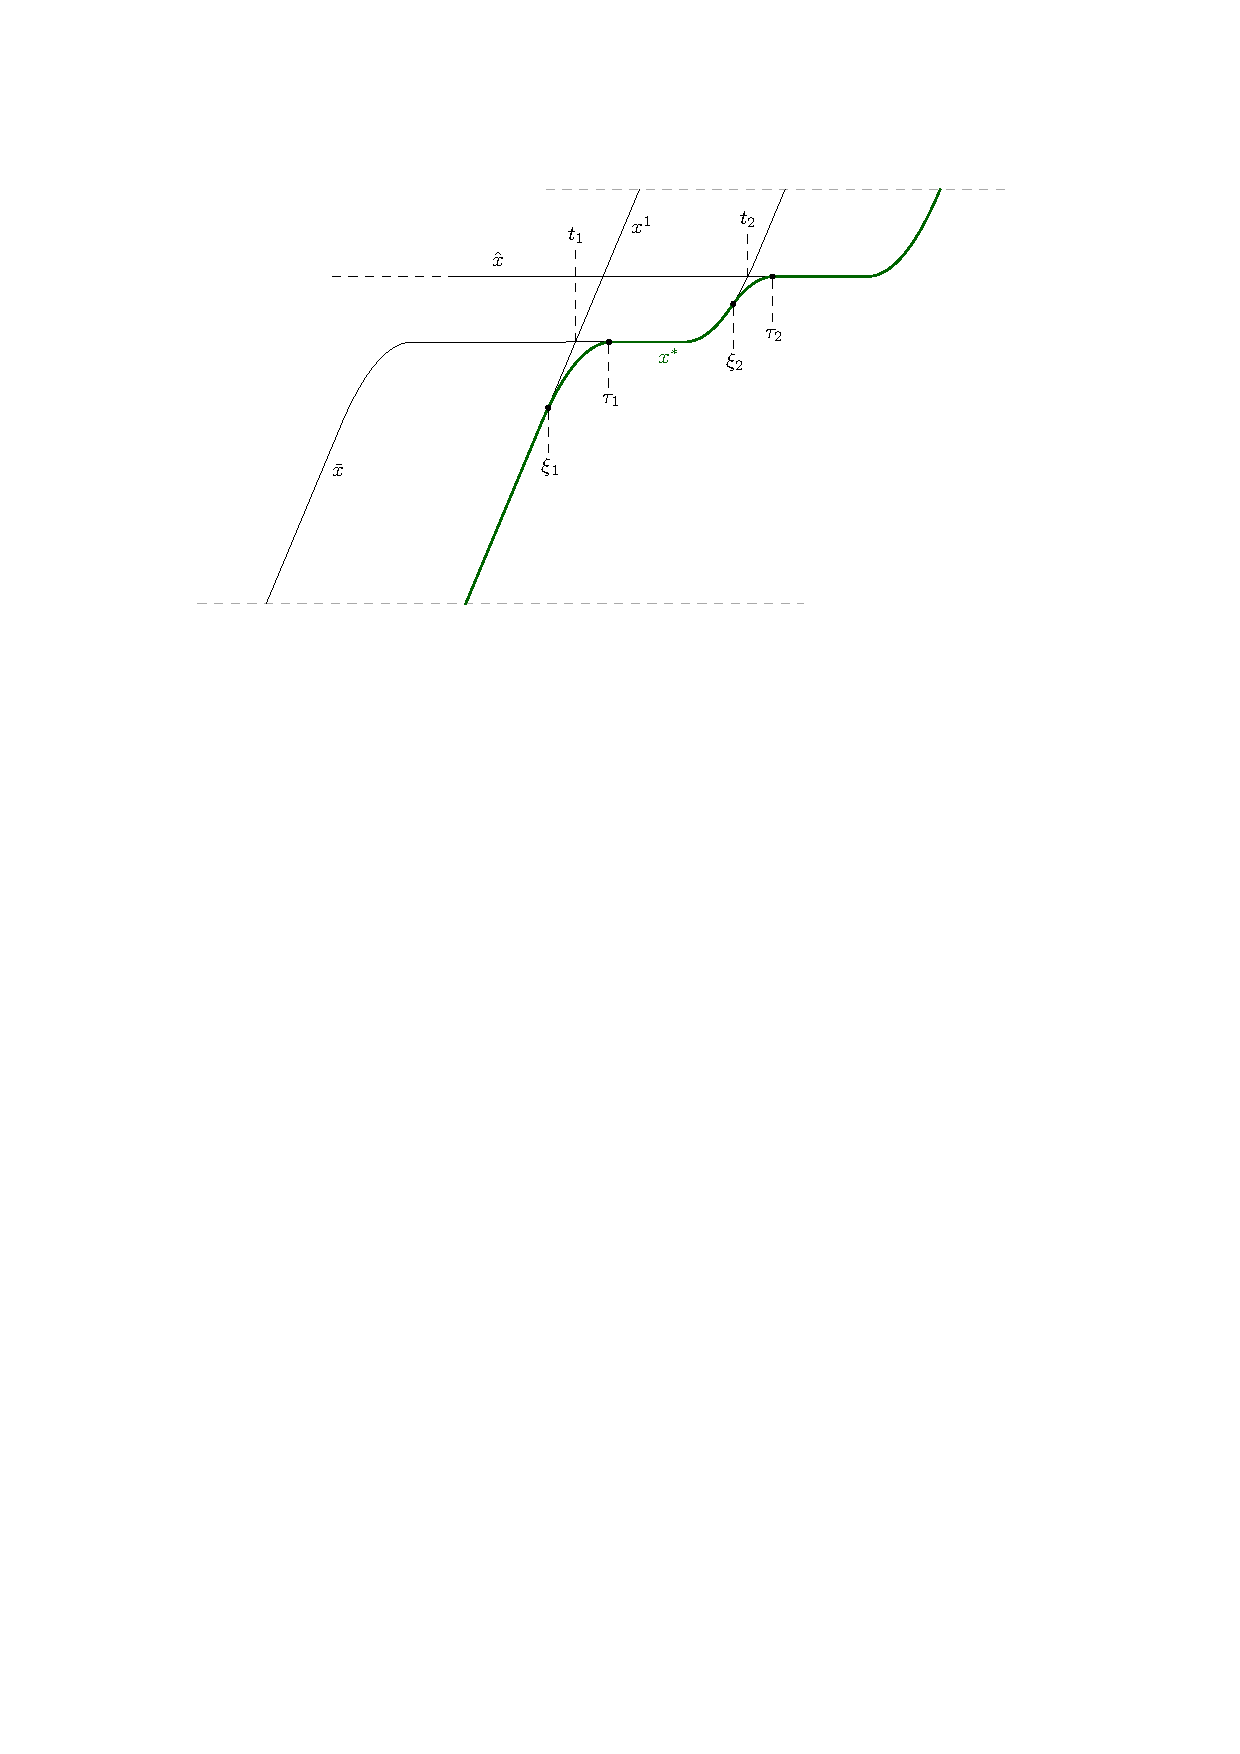
\includegraphics[scale=1]{figures/motion/rough/proof}
  \caption{Sketch of how the three boundaries are joined to form the
    optimal trajectory.}%
  \label{fig:theorem-proof}
\end{figure}

\begin{figure}
  \centering
  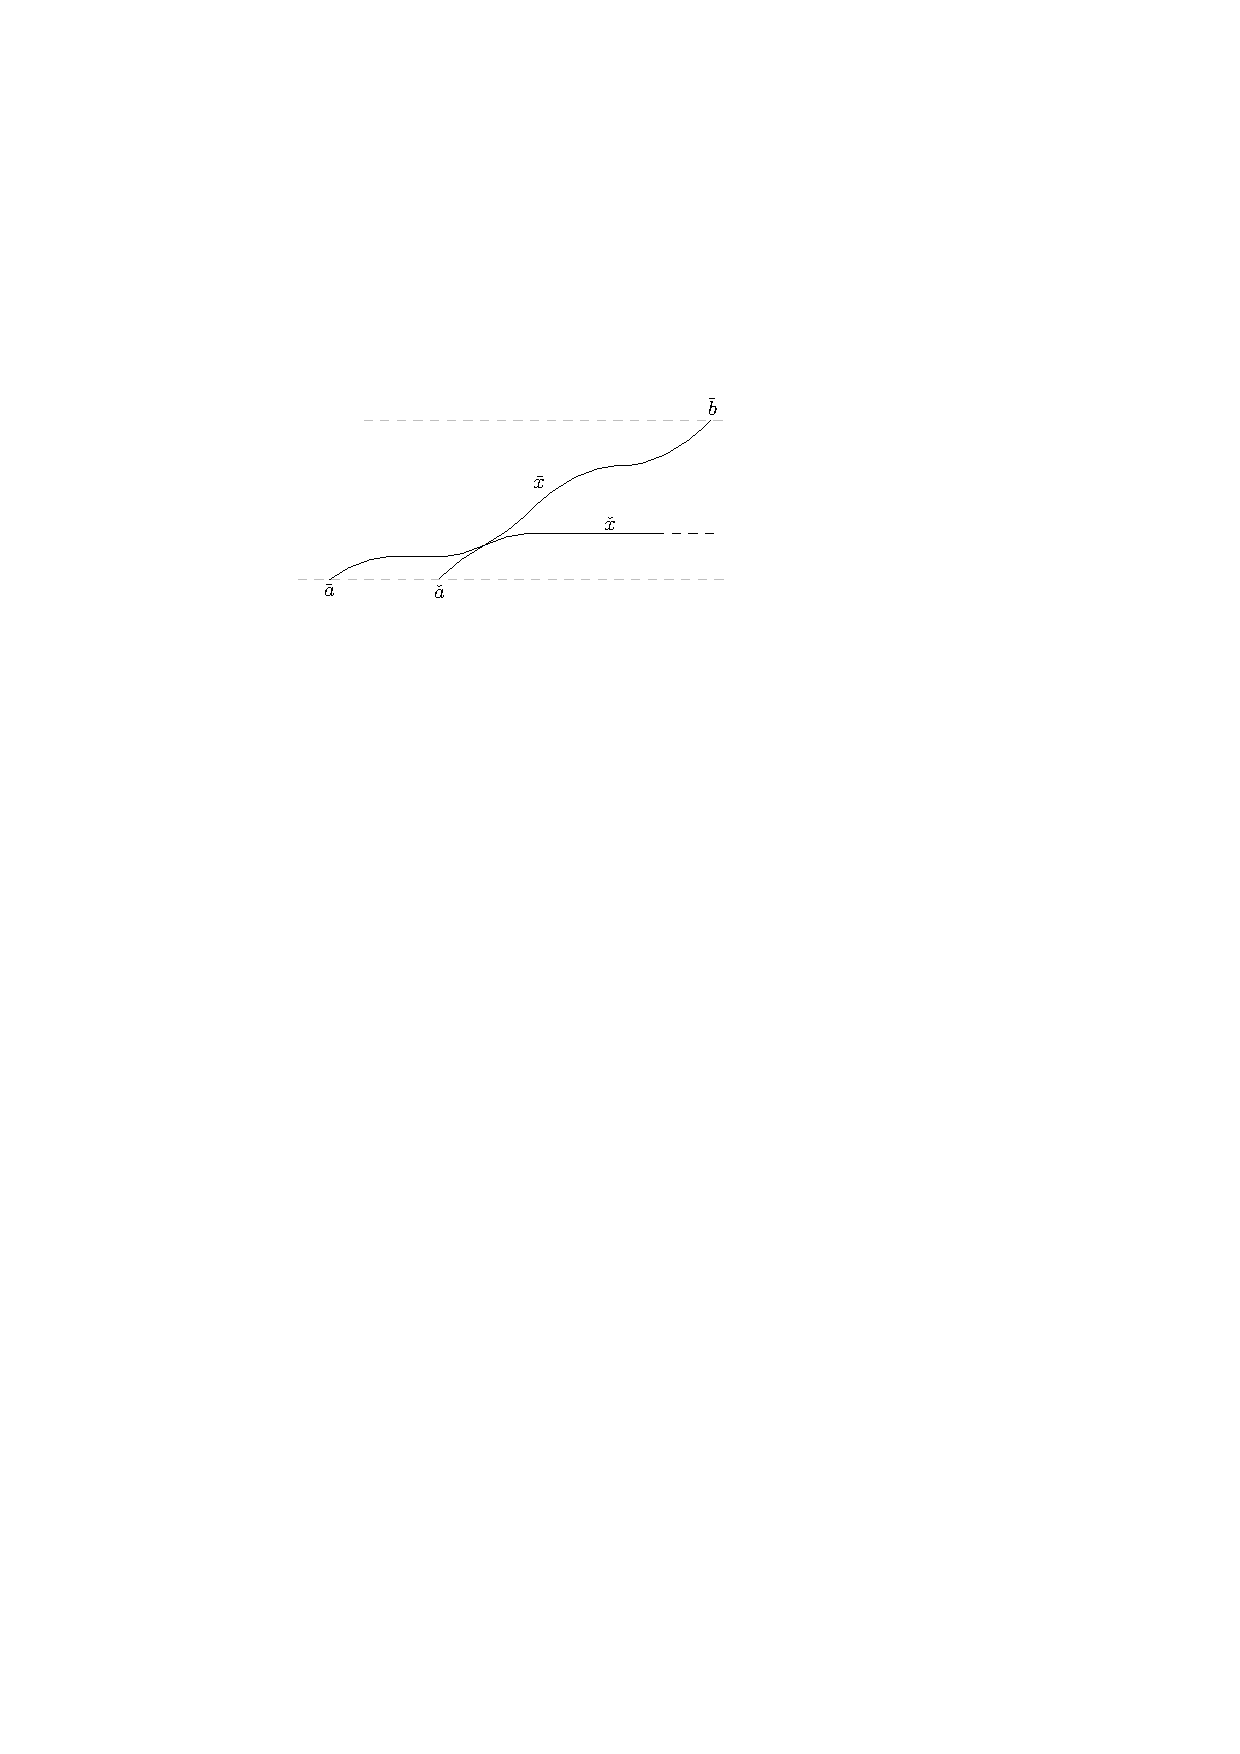
\includegraphics[scale=1]{figures/motion/rough/bufferconstraint}
  \caption{Illustration of ``buffer constraint''.}%
  \label{fig:bufferconstraint}
\end{figure}


\newpage
\appendix
\section{Miscellaneous}

\begin{lemma}\label{lemma:levelset}
  Let $f :\mathbb{R}^{n} \rightarrow \mathbb{R}^{m}$ be continuous and
  $y \in \mathbb{R}^{m}$, then the level set $N := f^{-1}(\{ y \})$ is a closed
  subset of $\mathbb{R}^{n}$.
\end{lemma}
\begin{proof}
  For any $y' \neq y$, there exists an open neighborhood $M(y')$ such that
  $y \notin M(y')$. The preimage $f^{-1}(M(y'))$ is open by continuity.
  Therefore, the complement
  $N^{c} = \{ x : f(x) \neq y \} = \cup_{y' \neq y} f^{-1}(\{y'\}) = \cup_{y' \neq y} f^{-1}(M(y'))$
  is open.
\end{proof}

\begin{lemma}
  Let $f : D \rightarrow \mathbb{R}^{n}$ be a function that is continuous in $t$
  and globally Lipschitz continuous in $x$. If there exists some closed
  rectangle $D \subseteq \mathbb{R} \times \mathbb{R}^{n}$ such that
  $(t_{0}, x_{0}) \in \interior D$, then there exists some $\varepsilon > 0$
  such that the initial value problem
  \begin{align}
    \label{eq:1}
    \dot{x}(t) = f(t, x(t)), \quad x(t_{0}) = x_{0}
  \end{align}
  has a unique solution $x(t)$ on the interval
  $[t_{0} - \varepsilon, t_{0} + \varepsilon]$.
\end{lemma}

{\color{Navy} The above existence and uniqueness theorem is also known as the
  Picard-Lindel{\"o}f or Cauchy-Lipschitz theorem. The above statement is based
  on the Wikipedia page on this theorem, so we still need a slightly better
  reference.}

\end{document}

% to enable the minted package
% Local Variables:
% TeX-command-extra-options: "-shell-escape"
% End:
